\documentclass[12pt,letterpaper]{book}

\usepackage{amssymb}
\usepackage{booktabs}
\usepackage[T1]{fontenc}
\usepackage[margin=1in]{geometry}
\usepackage{graphicx}
\usepackage[hidelinks]{hyperref}
\usepackage[mono=false]{libertine}
\usepackage{listings}
\usepackage{multirow}
\usepackage[numbers]{natbib}
\usepackage[libertine]{newtxmath}
\usepackage{subcaption}
\usepackage[svgnames]{xcolor}
\usepackage{xspace}

\newcommand{\chapquotes}{}
\newcommand{\Chap}{Chapter}
\newcommand{\chap}{chapter\xspace}
\newcommand{\paper}{thesis\xspace}
\newcommand{\Unix}{Unix\xspace}

\newcommand{\blacklist}[1][\xspace]{blocklist#1}
\newcommand{\whitelist}[1][\xspace]{allowlist#1}

\newcommand{\solb}[1]{{\color{magenta} TODO #1}}
\newcommand{\thesis}[1]{\solb{THESIS #1}}

\renewcommand{\contentsname}{Table of Contents}
\renewcommand{\lstlistlistingname}{List of Listings}

\lstset{captionpos=b,
	basicstyle=\ttfamily,
	keywordstyle=\color{Blue},
	commentstyle=\color{Green},
	columns=flexible,
	language=C++,
	upquote=true
}

\bibliographystyle{abbrvnat}

\newcommand{\ms}[1]{#1 ms}
\newcommand{\us}[1]{#1 \textmu{}s}

\newcommand{\attribchapquote}{}
\newcommand{\gapchapquote}{}
\newcommand{\widthchapquote}{3in}
\newenvironment{chapquote}[2][1in]{
	\renewcommand{\attribchapquote}{#2}
	\renewcommand{\gapchapquote}{#1}
	\vspace{-2in}
	\begin{flushright}
	{\Large ``}
}{
	{\Large ''} \\
	--- \attribchapquote \\
	\rule{\widthchapquote}{1pt}
	\end{flushright}
	\vspace{\gapchapquote}
}

\makeatletter
\let\includegraphics@\includegraphics
\renewcommand{\includegraphics}[2][]{\includegraphics@[#1]{\includegraphicsdir#2}}
\newcommand{\includegraphicsdir}{}

\let\input@\input
\renewcommand{\input}[2][.]{
	\renewcommand{\includegraphicsdir}{#1/}
	\input@{#1/#2}
	\renewcommand{\includegraphicsdir}{}
}

\let\figure@\figure
\let\endfigure@\endfigure
\let\includegraphixs@\includegraphics
\let\caption@\caption
\let\label@\label
\newenvironment{swallowfigures}{
	\renewenvironment{figure}{
		\renewcommand{\includegraphics}[2][]{}
		\renewcommand{\caption}[1]{}
		\renewcommand{\label}[1]{}
	}{
		\let\includegraphics\includegraphixs@
		\let\caption\caption@
		\let\label\label@
	}
}{
	\let\figure\figure@
	\let\endfigure\endfigure@
}

\let\section@\section
\newenvironment{swallowsections}{
	\renewcommand{\section}[1]{}
}{
	\let\section\section@
}

\let\subsection@\subsection
\newenvironment{swallowsubsections}{
	\renewcommand{\subsection}[1]{}
}{
	\let\subsection\subsection@
}

\newenvironment{promotesubsections}{
	\renewcommand{\subsection}[1]{\section@{##1}}
}{
	\let\subsection\subsection@
}
\makeatother

\newenvironment{abstract}{}{}

\newcommand{\mytableistoobig}{}

\begin{document}

\makeatletter
\let\label@\label
\let\ref@\ref
\newenvironment{namespacereferences}[1]{
	\renewcommand{\label}[1]{\label@{#1##1}}
	\renewcommand{\ref}[1]{\ref@{#1##1}}
}{
	\let\label\label@
	\let\ref\ref@
}
\makeatother

\frontmatter

\begin{titlepage}
\begin{center}
	\vspace*{\fill}

	\textbf{\Large Lightweight Preemptible Functions} \\
	A thesis \\
	\hfill \\
	{\large Sol Boucher} \\
	\today \\

	\vspace{1in}

	\textbf{Thesis committee:} \\
	David G.\@ Andersen, \textit{chair} \\
	Adam Belay \\
	Michael Kaminsky \\
	Brandon Lucia \\

	\vspace{\fill}

	\textit{Submitted in partial fulfillment of the requirements \\
	for the degree of Doctor of Philosophy} \\
	\hfill \\
	Computer Science Department \\
	School of Computer Science \\
	Carnegie Mellon University \\
	Pittsburgh, PA 15213 \\
\end{center}
\end{titlepage}

\cleardoublepage
\addcontentsline{toc}{chapter}{\contentsname}
\tableofcontents
\listoffigures
\addcontentsline{toc}{chapter}{\listfigurename}
\listoftables
\addcontentsline{toc}{chapter}{\listtablename}
\lstlistoflistings
\addcontentsline{toc}{chapter}{\lstlistlistingname}

\chapter{TODOs THESIS}


\section{Lessons for system builders (slides)}

Resuming is a useful feature that is cheap, but introduces concurrency.
Cannot get CPU time isolation without memory isolation.
Design abstractions modularly and with an eye to simple use cases (e.g., \textit{libgotcha} as a separate
runtime with a very small control API, things listed in the note on design).
Treat debuggability as a first-order concern (e.g., permit disabling features that interfere at
runtime, test and maintain support for running under debugging and diagnostic tools).


\chapter{Foreword}

Perhaps it is inevitable that when a nonfiction work reaches a certain length, it
begins to serve multiple purposes; if so, this document is no exception.  Yes, it is
a record of the ideas I have explored over the past years of my life.  But like any
thesis, it is also a lesson:\@ in summarizing my findings from these explorations, it
endeavors to save you from spending years of your own on the same topic.  And like
any good lesson, this one begins with an exercise...

With your permission, we will conduct a brief mindfulness activity.  At this moment,
and for however much longer you focus on this document, you mind will be occupied by
ideas.  Many of these ideas I will have put there.  Shortly, they will be ideas about
computer systems, but first let us consider:  How are the ideas getting to you?  You
are reading, but what does that mean?  Perhaps you are holding a printout or a bound
copy of this manuscript, or perhaps you have loaded it onto your personal computer,
tablet, phone, or hand terminal.  In any case, you have opened it to a particular
page, exposing your eyes to a sea of shapes arranged into nested clusters.  Your eyes
have gravitated to a cluster of particularly large shapes known as a ``chapter
title,'' then they have scanned across the page and sent a compressed representation
of each smaller ``word'' cluster of shapes to your brain, which has matched the
clusters of shapes to entries in your mental lexicon, then parsed them according to a
set of linguistic rules to infer their logical connections.  Then you have moved on
to the large ``paragraph'' clusters and processed each in turn, starting with the
first of its ``sentence'' clusters, and in so doing, learning what the next sentences
will be about.  Occasionally, something will go wrong at one of these steps and you
will backtrack and notice a missed word, or more closely examine a misidentified
word, or try a different parsing of the sentence, or reexamine the logical flow of
the paragraph.  You will usually not realize you are doing any of this, preferring
to think simply that you are \textbf{reading}.

The document you are reading is about computer systems, and like your brain, such
systems have many complexities.  If we as computer users had to describe the full
process for doing everything, we would never accomplish anything, so instead we
build \textbf{abstractions} for performing common tasks without examining the
underlying details.  Some would say that any computer systems research is
fundamentally about abstractions.  This particular work centers around an abstraction
for use by application programmers, who in turn work on top of other abstractions,
the most notable of which is software called the \textbf{operating system}.

In computing, as in life, one's fundamental goal is to accomplish some task using a
set of shared resources.  Someone must decide how to allocate these shared resources,
a role usually filled for a particular resource by a piece of software called its
\textbf{scheduler}.  One major responsibility of the operating system is to share
hardware resources such as the processor, the short- and long-term storage devices,
devices for user interaction, and network interfaces.  Among these, the one most
relevant to our discussion is the CPU scheduler, which manages the processor.

Despite itself being an abstraction that hides enormous complexity, a processor is
conceptually quite simple:\@ it receives a stream of simple \textbf{instructions}
telling it what to do, executing them in the order received and occasionally jumping
to a particular point elsewhere in the stream when so instructed.  The simplicity of
this model belies the infinite expressive power of programs constructed from such
instructions.  Indeed, programming at the instruction level is difficult not only
because the simplicity of the instructions make it verbose, but also because ad-hoc
jumps can be deceptively complicated to reason about.  Modern programmers usually
write software in programming languages that provide so-called ``structured control''
abstractions for performing common, formulaic sequences of jumps.

The most fundamental abstraction composing a structured program is the
\textbf{function}:\@ a section of code that expects zero or more input data, performs
some computation, and generates zero or more output data.  One function can call
another, which automatically transfers the input data and jumps to the start of that
function's code.  Later, when the end of its code is reached, the function
automatically jumps back to the program point just after it was called and transfers
its output data back.  Notice that a function call is \textbf{synchronous}; that is,
the function runs to completion before the calling function continues to run.
Because such sequential execution matches the processor's inherent behavior, sharing
the processor between functions is trivial and requires no scheduler.

Of course, an important feature of modern computers is the ability to work on
multiple tasks alongside each other, such as reading a document and composing an
outline or notes.  Operating systems manage such situations by providing an
abstraction called a \textbf{process}, or independent task.  Each process is isolated
from the others on the system and cannot access their data.  Furthermore, processes
exhibit a property known as \textbf{concurrency} wherein their executions can
interleave such that one process executes some of its code ``in the middle of''
another process's work.  (Think of momentarily putting your notetaking on hold to
scroll down in the document you're reading.)

Because isolation prevents processes from calling each other's functions directly,
switching between processes requires a scheduler to transfer control of the
processor.  Specifically, the processor must stop executing the running process and
start running the operating system's CPU scheduler code, which then performs an
action called a \textbf{context switch}:\@ it saves a checkpoint of that process and
restores the other process, resuming it from the state in which it last left off.
The conceptually simpler way for this transition to happen is \textbf{cooperative}
multitasking, in which the former process voluntarily gives up control of the
processor by explicitly telling the operating system to give someone else a turn.
Unfortunately, it is not safe to assume a process will eventually cede its processor,
as it may never decide to do so, through either misbehavior or malice.  Such a
scenario would render the rest of the programs unusable.

Fortunately, processors have a low-level mechanism for spontaneously changing which
instruction they are executing known as a \textbf{timer interrupt}.  Every so often,
the processor jumps into the OS scheduler from whatever code it is currently
executing.  Since it is now has the use of the processor, the scheduler can decide
whether to jump back to that same program or context switch to a different one, a
decision that is usually made based on how long the former program had been running
since the last context switch.  This style of process scheduling is known as
\textbf{preemptive} multitasking because the operating system initiates it by
actively pausing the running process.

Recent decades have seen the introduction of multicore computers that have more than
one processor, creating the opportunity for the operating system to schedule a
different process on each.  Such processes exhibit \textbf{parallelism}:\@ they
actually run at the same time.  Parallelism is also an attractive feature for
application programmers because by carefully restructuring their programs, they can
route some of their work to each processor, thereby speeding up portions of their
program's run.  Unfortunately, fitting such programs into operating systems' existing
process model was cumbersome.

To better accommodate parallel programs, operating systems introduced a hybrid
abstraction called a \textbf{thread}.  Like processes, threads can be both concurrent
and parallel.  Unlike processes, though, threads must share data to effectively
work together on a single task, so the threads within a process are not isolated from
one another.  It turns out that the simultaneous presence of concurrency and shared
data introduces fundamental challenges that make it difficult to write correct
programs due to a class of bugs informally known as race conditions.  Although safe
concurrency is a popular area of study, challenges remain particularly in systems
containing components that predate the parallel programming paradigm.  More detailed
coverage of safe concurrency and backwards compatibility as they relate to this
thesis work appears in chapters~\ref{chap:libinger} and \ref{chap:libgotcha},
respectively.

The lack of isolation between threads permits the programmer to spawn a thread in
much the same way they would call a function:\@ in most programming languages, they
place the code they want to execute on the new thread in its own function, but
instead of calling it directly, they pass it to a special wrapper function.  The
wrapper sets up the thread and begins running the programmer's custom thread thereon.
However, in an important break from functions, threads are \textbf{asynchronous} like
processes.  The wrapper function returns almost instantly, even if the thread is
still running in the background.  As with processes, this property means there must
be a scheduler to decide which application code each processor should run.  Note
that for the sake of this discussion, we are assuming this is the operating system's
CPU scheduler; however, this is not always the case and sometimes a custom scheduler
runs as part of the application itself, a configuration that is addressed in detail
in chapter~\ref{chap:libturquoise}.

Introducing additional scheduler dependencies on an application has important
functionality and performance ramifications for two fundamental reasons.  First, the
scheduler's placement behind an abstraction decouples it from the program's logic,
thereby imposing one or more levels of communication barrier that reduce its
understanding of the particular application's needs, often resulting in a brittle
policy ill suited to the workload.  For instance, few preemptive schedulers provide a
way for an application to customize the timer interrupt interval, even when supported
by the hardware.  Second, every scheduler works by running its own code to make
decisions about how to allocate a resource.  Because it does not represent useful
work from the application's perspective, time spent this way is pure overhead, and it
follows that introducing unnecessary scheduling necessarily reduces performance.

Threads represent the standard application for exploiting preemption within an
application.  However, reminiscent of how processes were cumbersome to use for
parallel programming, threads are ill suited to some use cases of preemption.  For
one thing, programmers who do not need parallelism are led to build their synchrony
atop asynchrony, thereby introducing a useless scheduler dependency.  For instance,
when calling a helper function but needing a result by a specific deadline is tempted
to spawn the function on its own thread, then immediately wait for the thread to
finish, a task better accomplished on the same thread.  Furthermore, although they
support pausing code mid-execution, threads make it very difficult to cancel
in-progress work that is no longer needed at all.

Fortunately, the tendency to use threads for application-level preemption is not
because the operating system does not expose hardware features such as timers.
Rather, it is because such features are presented as very low-level abstractions that
perform hardware-style unstructured jumps rather than using language-style structured
control and abstracting away the details of context switching.  We therefore propose
a new abstraction for easy preemption within an application, but show that it can be
implemented on top of the existing operating system.



\mainmatter

\section{Introduction}
\label{sec:intro}

As the scope and scale of Internet services continues to grow, system designers
have sought platforms that simplify scaling and deployment.
Services that outgrew self-hosted servers moved to datacenter racks, then
eventually to virtualized cloud hosting environments.
However, this model only partially delivered two related benefits:
\begin{enumerate}
\item Pay for only what you use at very fine granularity
\item Scale up rapidly on demand
\end{enumerate}

\noindent
The VM approach suffered from relatively coarse granularity:  Its atomic compute unit
of machines were billed at a minimum of minutes to months.  Relatively long startup
times often required system designers to keep some spare capacity online to handle
load spikes.

These shortcomings led cloud providers to introduce a new model, known as
serverless computing, in which the customer provides \textit{only} their code,
without having to configure its environment.   Such ``function as a service''
(FaaS) platforms are now available as AWS Lambda~\cite{www-amazon-lambda}, Google
Cloud Functions~\cite{www-google-cf}, Azure Functions~\cite{www-microsoft-af}, and
Apache OpenWhisk~\cite{www-apache-openwhisk}.  These platforms provide a model in
which: (1)  user code is invoked whenever some event occurs (e.g., an HTTP
API request), runs to completion, and nominally stops running (and being
billed) after it completes; and (2)  there is no state preserved between
separate invocations of the user code.  Property (2) enables easy auto-scaling
of the function as load changes.

Because these services execute within a cloud provider's
infrastructure, they benefit from low-latency access to other cloud
services.  In fact, acting as an access-control proxy is a recurring microservice
pattern:\@ receive an API request from a user, validate it, then access
a backend storage service (e.g., S3) using the service's credentials.

In this paper, we explore a design intended to reduce the tension between two of
the desiderata for cloud functions:\@ low latency invocation and low cost.  Contemporary
invocation techniques exhibit high latency with a
large tail; this is
unsuitable for many modern distributed systems which involve
high-fanout communication, sometimes performing thousands of
lookups to handle each user request.  Because user-visible response time often
depends on the tail latency of the slowest chain of dependent
responses~\cite{Dean:cacm2013}, shrinking the tail is crucial~\cite{Jalaparti:sigcomm2013,
Xu:nsdi2013,Li:socc2014,Jeon:asplos2016}.

Thus we seek to reduce the invocation latency and improve predictability, a
goal supported by the impressively low network latencies available in modern
datacenters. For example, it now takes $<20\mu{}s$ to perform an RPC between two
machines in
Microsoft Azure's virtual machines~\cite{Firestone:nsdi2018}. We believe,
however, that fully leveraging this improving network performance will require
reducing microservices' invocation latencies to the point where the network is
once again the bottleneck.

We further hypothesize---admittedly without much proof for this chicken-and-egg
scenario---that substantially reducing both the latency and cost of running
intermittently-used services will enable new classes and scales of applications
for cloud functions, and in the remainder of this paper, present a design that
achieves this.  As Lampson noted, there is power in making systems 
``fast rather than general or powerful''~\cite{Lampson1983}, because fast
building blocks can be used more widely.

Of course, a microservice is only as fast as the slowest service it relies on;
however, recall that many such services are offered in the same clouds and
datacenters as serverless platforms. Decreasing network latencies will push
these services to respond faster as well, and new stable storage
technologies such as 3D XPoint (projected to offer sub-microsecond reads and
writes) will further accelerate this trend by offering lower-latency storage.

In this paper, we propose a restructuring of the serverless model centered around
low-latency: \textit{lightweight microservices} run in \textit{shared processes}
and are isolated primarily with language-based \textit{compile-time guarantees} and
\textit{fine-grained preemption}.

%% \subsection{Not yet rewritten}

%% At the time of writing, AWS Lambda, Azure Functions, and Google Cloud Functions
%% cap instance execution time to 5--10 minutes.

%% \solb{AK: I see you touched this recently.  Do you still want to see us say it (and
%% where)?  I currently mention penultimate section of Motivation and related work that
%% providers presently impose a limit, without actually saying what it is.}
%% \mk{This subsection seems out of place.}

\chapter{Function calls with timeouts}
\label{chap:functions}

\ifdefined\chapquotes
\begin{chapquote}{Isaac Asimov, \textit{The Gods Themselves}}
`Does everyone just believe what he wants to?' \\
`As long as possible.  Sometimes longer.'
\end{chapquote}
\fi

\begin{figure}
\begin{center}
\includegraphics[width=0.65\columnwidth]{functions/figs/progsupport}
\end{center}
\caption{Taxonomy of support for library code.  It is difficult to determine whether
a library is fully reentrant, so in practice we always
apply one of the two mitigations.  Library copying is used by default, but deferred
preemption is needed to preserve the semantics of \texttt{malloc()} and users of
uncopyable resources such as file descriptors or network adapters.}
\label{fig:progsupport}
\end{figure}

\begin{swallowsections}
\begin{swallowfigures}
\input[functions]{intro}
\end{swallowfigures}
\end{swallowsections}
\input[functions]{related}
\input[functions]{inger_inger}

\input[functions]{inger_noninger}

\section{Automatic handling of shared state: \textit{libgotcha}}

\begin{swallowsubsections}
\input[functions]{inger_gotcha}
\end{swallowsubsections}
\input[functions]{inger_pause}

\chapter{Nonreentrancy and selective relinking: \\ the \textit{libgotcha} runtime}
\label{chap:libgotcha}

\ifdefined\chapquotes
\vspace{-1in}
\begin{chapquote}[1.5in]{James S.\@ A.\@ Corey, \textit{Nemesis Games}}
`Alien superweapons were used,' Alex said, walking into the room, \\
sleep-sweaty hair standing out from his skull in every direction. \\
`The laws of physics were altered, mistakes were made.'
\end{chapquote}
\fi

In Section~\ref{sec:libinger:reentrancy}, we saw that it is not safe in general for a
preemptible function to call into stateful code that was written without the
preemptible function abstraction in mind.  However, such code is prolific in the
modern systems stack, and in order to support interoperability with it, we need to
automatically transform the program to fix the safety hole.  This chapter covers a
novel software system designed to do just that, dubbed \textit{libgotcha}.

\begin{figure}
\begin{center}
\includegraphics[width=0.7\columnwidth]{figs/procimg_perobj}
\end{center}
\caption{Layout of a typical module within the process image.  \textbf{Bold} sections
contain program data; \textit{italicized} ones contain metadata for the runtime.}
\label{fig:procimgobj}
\end{figure}

\begin{promotesubsections}
\begin{swallowsections}
\input[functions]{gotcha_gotcha}
\end{swallowsections}
\end{promotesubsections}
\hspace{-2.5em}
Our discussion in this chapter uses \textit{libinger} as a motivating example of a
\textit{libgotcha} user, as this configuration was the inspiration for the runtime's
creation.  However, we have found that the described techniques to be general and
equally relevant to applications besides timed functions.  As such,
\textit{libgotcha} exposes a general API that allows any \textbf{control library} to
configure its behavior for the process.  We give more details later in the chapter,
and study other examples of control libraries in Chapter~\ref{chap:safety}.


\section{A brief tour of linking}
\label{sec:libgotcha:link}

We begin with background about linking, a two-stage process that ultimately produces
an in-memory \textbf{process image} containing a program's code, all the data it
needs to execute, and the code and data of all its dependencies.  Linking operates on
\textbf{object files} that can take the form of either an \textbf{executable} or a
\textbf{shared library}.  Once a program is running, its process image contains a
region corresponding to each loaded object file.  We will refer to each such region as
a \textbf{module}, regardless of whether it corresponds to an executable or a shared
library.  Each module is divided into logical \textbf{sections}, each containing a
particular type of information.  Figure~\ref{fig:procimgobj} shows a typical module's
layout; notice that it contains both data corresponding to the source code and
generated metadata for runtime consumption.

The linking process occurs in two parts.  Static linking occurs at compile time and
forms the last step of the traditional build process.  Dynamic linking occurs at a
phase of runtime we will refer to as \textbf{load time}, because it starts before the
program has been loaded from disk or the language runtime initialized.


\subsection{Static linking}

Invoking the \texttt{cc} compiler driver does more than just compile C code:\@ it
runs the C preprocessor \texttt{cpp}, the C compiler (\texttt{cc1} in GCC's case),
then the static linker \texttt{ld}.

The output of the second step is a relocatable object file containing code and data
with referenced addresses identified by named \textbf{symbols}.  In a relocatable
object file, symbol \textbf{references} such as instructions making function calls
or accessing global variables are encoded with a null address as a placeholder.  Each
object file contains a \textbf{relocation table} in a separate section that
associates each placeholder with a symbol name, which may or may not be located in
the same file.  Each object file also contains a \textbf{symbol table} to identify
the symbols it defines and associate them with the file offset of their definition.
Note that only non-\texttt{static} C symbols generate global symbol table entries
that can be referenced from other object files; this keyword is confusingly named and
does not refer to static linking.  The compiler's ultimate output is one relocatable
object file for each source file.

The static linker is responsible for combining one or more relocatable object files
into a single executable or shared library, where either type of output file is
ready for loading into memory for execution.  This process consists of verifying that
there is a definition corresponding to each symbol reference, unifying the sections
across object files and choosing a final address (or relative address) for each
symbol, encoding the chosen addresses at the location recorded in each relocation
table entry, and writing the resulting file to disk.  This output file does not
preserve the relocation table because the linker has already fixed the null pointers
it described.  The file does contain a symbol table because it can be useful for
debugging (e.g., to generate stack traces), but this can be removed using the
\texttt{strip} utility without affecting the program semantics.

With the exception of macOS, most modern Unix systems use ELF (Executable and
Linkable Format) object files.  One advantage of this format is that executables and
shared libraries are themselves ELF object files.


\subsection{Dynamic linking}
\label{sec:libgotcha:dylink}

Static linking allows programs to reuse ``libraries'' of precompiled object files,
but each program must be built with its own copy of all its libraries within the
executable.  This means that every time an application is loaded, its libraries' code
and data must be read back from disk, even if another running program uses the same
libraries; it also means that updating a library requires recompiling all dependent
programs installed on the system.  Dynamic linking solves both problems by separating
libraries into separate files that are not read until the executable runs.\footnote{
Specifically, this separation obviates the need to read the files from disk multiple
times because the runtime maps them into the process image using the \texttt{mmap()}
family of system calls.  The kernel tracks regions that are already mapped and serves
recurring requests from memory instead of disk, mapping to the same physical memory
if the pages are read-only or creating copy-on-write page mappings otherwise.}

By splitting libraries into their own files, dynamic linking introduces a build-time
challenge:\@ the relative position and offset of modules cannot be known until
runtime.  As such, rather than performing the relocations for inter-module symbol
references, the static linker leaves the placeholder addresses and adds a separate
dynamic relocation table and dynamic symbol table into the output object file.
Unlike the tables used for static linking, these are needed to launch the program, so
tools such as \texttt{strip} leave them in place.  For executables, the linker also
writes the path to an ``interpreter'' program into the ELF program header.

When asked to load a program that declares an interpreter, the kernel loads and jumps
to the interpreter instead of the executed program.  Usually, this interpreter is the
system \textbf{dynamic linker}, traditionally named \texttt{ld.so}.  Before jumping
into the program code, the dynamic linker loads all the modules and processes the
entries in each of their dynamic relocation tables.  The relocations are not
restricted to modifying writeable memory:\@ they can update constant global data and
even executable instructions.  Even if they leave the code unchanged, its position
relative to the rest of the module matters.  These points are critical to our use
case, as they mean that in order to duplicate modules' data, we must also duplicate
their code.

Another consequence of relocations being able to alter read-only memory is that the
dynamic linker must change the page protections of these regions after it is finished
processing relocations.  To support this, the compiler splits up module components
into fine-grained sections by purpose.  Non-\texttt{const} global variables are
placed in the \texttt{.data} and \texttt{.bss} sections, which must remain writeable
at runtime and therefore require no special action.  In contrast, \texttt{const}
globals are split between the \texttt{.rodata} and \texttt{.data.rel.ro} sections
based on whether they require relocation; in the latter case, the dynamic linker
marks the pages read-only before passing control to the program.

If relocations routinely modified scattered locations throughout the executable
\texttt{.text} section, the dynamic linker would have to change page protections on
most or all of each module's code pages.  This would require a lot of system calls,
but it would also require copy-on-write code mappings, preventing instruction cache
hits between processes using the same library.  To avoid these problems, the compiler
indirects references to dynamic symbols via a structure called the GOT (Global Offset
Table).

\begin{figure*}
\begin{minipage}{\textwidth}
	\includegraphics[width=\textwidth]{figs/gotables-crop}
	\subcaption{Reading a library's global variable: \texttt{size\_t tmp = data;}}
	\label{fig:dytabs:got}
	\end{minipage}

	\begin{minipage}{\textwidth}
	\includegraphics[width=\textwidth]{figs/pltables-crop}
	\subcaption{Calling an eagerly-resolved library function: \texttt{fun()}}
	\label{fig:dytabs:plt}
	\end{minipage}

	\begin{minipage}{\textwidth}
	\includegraphics[width=\textwidth]{figs/jstables-crop}
	\subcaption{Calling a lazily-resolved library function.  In step \textcircled{5},
	the dynamic linker memoizes the resolved address into the GOT; subsequent calls
	proceed as above.}
	\label{fig:dytabs:lazy}
	\end{minipage}
\caption{Table references required to reference global symbols in dynamically-linked
programs}
\label{fig:dytabs}
\end{figure*}

The GOT is a table of relocated pointers to symbol definitions, whether those
definitions are within the same module or in a different one.  To avoid generating
code pages that require relocations, the compiler compiles each reference to or
dereference of non-\texttt{static} global data into a position-independent load of
the corresponding pointer from the GOT.  Figure~\ref{fig:dytabs:got} shows an example
of the two instructions and one table reference needed for a dereference.  A
reference would generate only the first \texttt{mov} instruction, as would taking a
pointer to a function.

Calling a global function works differently and relies on another indirection
structure called the PLT (Procedure Linkage Table), which contains code instead of
pointers.  For each call to a non-\texttt{static} function, the compiler generates a
position-independent call to a PLT entry corresponding to the function being called.
It generates a PLT entry, which is a short sequence of instructions that loads the
pointer to the real definition from the GOT, then executes and indirect jump to that
location.  Figure~\ref{fig:dytabs:plt} shows an example function call.  As with GOT
entries, there are PLT entries for functions defined both within and outside the
referencing module.

Not all function calls are this simple.  To save the dynamic linker some work at load
time, many function calls resolve lazily on their first execution.  Such resolution
involves a series of jumps designed to memoize the address so that subsequent calls
to the function from the same module do not repeat the expensive lookup.
Figure~\ref{fig:dytabs:lazy} shows the effect of the first call to such a
function:\footnote{This representation is slightly simplified for brevity.  In
practice, it is undesirable to hardcode the address of a dynamic linker function into
each module.  Therefore, instead of jumping directly to the symbol resolver, the slow
lookup path jumps to a dedicated PLT stub that loads its address from another GOT
entry.  Technically, there are separate identifiers for the symbol and the module,
each pushed to the stack by one of these two involved PLT stubs.}  \textcircled{1}
The program calls the PLT stub, just as it would for an eagerly-resolved function.
\textcircled{2} The PLT stub is longer (three instructions instead of one), but still
begins with an indirect jump to the pointer found in the corresponding GOT entry.
\textcircled{3} The GOT entry initially contains the address of the PLT stub's second
instruction, so the indirect jump is a no-op and merely advances the instruction
pointer.  \textcircled{4} The rest of the PLT stub pushes a constant identifying the
module and symbol onto the stack, then jumps to a symbol-lookup function in the
dynamic linker.  \textcircled{5} After looking up the address of the symbol's
definition, the dynamic linker uses the identifier from the stack to find and update
the GOT entry in the calling module.  \textcircled{6} The dynamic linker jumps to the
symbol in the defining module.  Because the GOT entry has been updated, future calls
proceed exactly like eagerly-resolved ones and jump directly to the symbol definition
from the first instruction of the PLT stub.  Of course, the GOT entries associated
with lazy PLT stubs must be writeable at runtime; this is why
Figure~\ref{fig:procimgobj} shows the GOT as split between two sections.

The dynamic linker performs all relocations and other standard module setup
automatically at load time, but the initialization process is pluggable.  In
particular, modules can include \textbf{constructor} functions to be invoked before
control is transferred to the runtime and ultimately the program's main function.  As
we will see, our work leverages this feature to override certain relocations at the
conclusion of load time.


\begin{promotesubsections}
\begin{swallowsections}
\input[functions]{gotcha_namespaces}


\input[functions]{gotcha_libsets}

Thus, selective relinking is selective in two ways, only affecting execution when the
next libset differs from the current libset and the program references a dynamic
symbol defined in a module that is not currently executing on that thread.

\solb{Expand interface listing and add comments with section references}
\end{swallowsections}
\end{promotesubsections}


\subsection{Detecting cross-module symbol references}

Identifying which GOT entries correspond to cross-module symbol references is a
multi-step process:
First, we traverse the relocation table for each loaded module, cross referencing
each of its relocation entries against the local module's symbol table.  If the
symbol table does not contain a definition matching the relocation entry's target, we
conclude that the relocation must correspond to a cross-module call.  Otherwise, we
check the address in the GOT entry corresponding to the relocation:  If this address
is outside the memory bounds of the current module, it is a cross-module call.
Otherwise, if this address matches the one from the symbol table entry, it is not a
cross-module call, and should be skipped.  The trickiest case is when the GOT entry
does not match but does point somewhere within the current module, since this means
it probably still refers to the PLT stub (because the symbol reference is lazy and
has not yet been resolved, as covered at the end of
Section~\ref{sec:libgotcha:dylink}).  In this case, we resolve the symbol early,
update the GOT entry, and recheck whether it resolved to the local definition to
determine whether it is a cross-module call.


\begin{promotesubsections}
\begin{swallowsections}
\input[functions]{gotcha_init}
\end{swallowsections}
\end{promotesubsections}

If a preemptible function is canceled rather than being allowed to return, execution
might be interrupted within a call to a library function.  For this reason,
\textit{libgotcha} must treat the libset's shared state as corrupted; it provides the
\texttt{libset\_reinit()} function shown in Listing~\ref{lst:gotchaapi} to allow
control libraries to inform it of such a situation so it can \textbf{reinitialize}
the libset before returning it to the pool.

Our early approach to reinitialization was to unload and reload all objects in the
libset by calling \texttt{dlclose()} followed by \texttt{dlmopen()}.  While this
approach theoretically allowed us to delegate the work to the dynamic linker, in
practice it introduced significant complications.\footnote{Most notably, some shared
libraries are marked with a special configuration flag, \texttt{DF\_1\_NODELETE},
which prevents the dynamic linker from ever removing them once they have been loaded.
Because almost all libraries depend on libc, the presence of even one such library
would prevent us from reinitializing a libset.  The flag is mostly used on libraries
that need to monkey-patch some other loaded library, such that the two subsequently
have a circular dependency.  Fortunately, this was not generally a problem for us
because when we unload one library from a libset, we then unload the rest.  Whenever
we encountered a \texttt{NODELETE} object file, we would make a special copy with the
flag cleared, for loading into every namespace except the main one.}  Worse, it
required the dynamic linker to reprocess all relocations throughout the libset, which
introduced prohibitive runtime latency.  We measured reinitialization taking almost 5
ms (over 10 million cycles on modern processors) on even small minimal example
programs~\cite{boucher:atc2020}.  With such delays, the only reasonable way for the
control library to handle cancellation was to delegate the reinitialization to a
separate thread to take it off the critical path; of course, this approach only works
as long as the number of libsets is not a bottleneck.

We have since redesigned reinitialization around a significantly faster approach:\@
checkpointing only portions of each module.  The key insight is that, as we saw in
Section~\ref{sec:libgotcha:link}, only some sections are writeable at runtime.  We
can therefore assume that these are the only memory regions of each module that can
change.  After populating the libset pool at application start, \textit{libgotcha}
iterates through each module of each libset and makes a backup copy of all its
writeable regions.  When a control library calls \texttt{libset\_reinit()},
\textit{libgotcha} restores each such region from the backup before returning the
affected libset to the pool.  We summarize this approach, which has reduced the
latency of reinitialization by two orders of magnitude, in
Figure~\ref{fig:reinit}.\footnote{We will address the version watermark alluded to
therein later in this chapter.}  To avoid having to repeat relocations and rerun any
module constructors, we capture the backup after dynamic relocation is complete and
all constructors have run; the tradeoff is that we actually have to copy memory,
rather than leveraging copy on write to later restore to the version on disk.

\begin{figure}
\includegraphics[width=\columnwidth]{figs/reinit-crop}
\caption{Libset reinitialization to support asynchronous cancellation}
\label{fig:reinit}
\end{figure}


\section{Selective relinking}

Most of the complexity of \textit{libgotcha} lies in the implementation of selective
relinking, the mechanism underlying libset switches.  To establish the libset
abstraction, it must arrange to conditionally intercept cross-module symbol
uses based on the currently-configured next libset.

As we saw in Section~\ref{sec:libgotcha:dylink}, whenever a program references a
dynamic symbol, it looks up the address of the definition in a data structure called
the global offset table (GOT).  Selective relinking works by shadowing the
GOT.\footnote{Hence the name \textit{lib\textbf{got}cha}.}  Just after the dynamic
linker populates the GOTs, \textit{libgotcha} replaces every entry that should
sometimes trigger a libset switch with a fake address.  It stores the original
address in its shadow GOT, which is organized by the libset that houses the
definition.  The fake address used depends upon the type of symbol:


\subsection{Intercepting function calls}

When setting up selective relinking, we do not know whether a particular function
call needs to be rerouted until runtime.  However, the fact that dynamic function
calls consult the GOT to determine which code to execute makes it efficient and
relatively straightforward to receive a notification whenever they occur.  To set
this up, at load time, we replace each such cross-module GOT entry with the address
of the special \textit{libgotcha} function \texttt{procedure\_linkage\_override()}.
Whenever the program tries to call one of the affected functions, control transfers
to this function instead; it then checks the thread's next libset, looks up the
appropriate symbol definition in the shadow GOT, and jumps to that location.  Because
\texttt{procedure\_linkage\_override()} runs between the caller's \texttt{call}
instruction and the real function, it is written in assembly to avoid clobbering
registers (e.g., those used for argument passing).

There is one major complication that necessitates an additional level of indirection
beyond what we have described.  Recall from the eagerly-resolved function calling
sequence in Figure~\ref{fig:dytabs:plt} that each function call site calls a
one-instruction PLT stub that performs an indirect jump to the real definition via
the GOT.  This means that if we simply replaced all the GOT entries with the address
of \texttt{procedure\_linkage\_override()}, that function would not know which GOT
entry it was being called via, and therefore which symbol to look up.  Instead, we
introduce our own table of executable stubs called the PLOT (Procedure Linkage
Override Table).  Unlike PLT entries, ours always push an identifier indicating which
function is being called.  For this, we use indices into a custom data structure
called the GOOT (Global Offset Override Table), which stores enough information to
find the symbol's shadow GOT entries while being practical to traverse in handwritten
assembly code.  Figure~\ref{fig:override} summarizes the modified dynamic function
call sequence under selective relinking.

\begin{figure}
\includegraphics[width=\textwidth]{figs/tables-crop}
\caption{Calling an eagerly-resolved library function under selective relinking}
\label{fig:override}
\end{figure}

A subtle but important point about dynamic linking is that pointers to the same
definition must compare equal, regardless of where they are obtained.  For instance,
the reader might notice that invocation is not the only thing a program can do with a
function:\@ it might also pass around the function's address.  In fact, after taking
the address, it could pass it to code within a different module, which might need to
know whether a third module passed a pointer to the same function.  To support such
comparisons, the compiler exclusively generates eagerly-resolved relocations for any
function that a particular module obtains a pointer to.  This way, the \texttt{mov}
to retrieve the pointer always finds the resolved address of the real definition in
the GOT.  To avoid breaking pointer comparison, \textit{libgotcha} associates each
PLOT entry with its function's definition, not its call site or calling module.  This
provides correct comparison semantics because all references to a particular function
receive the same pointer to a particular PLOT entry, and although this pointer
technically refers to the corresponding symbol's definitions in all libsets, at any
one time all calls to it will only resolve to the definition in the next libset.
Since at any given time there can only be one next libset, calls to pointers that
compare equal always refer to the same copy of the definition.

The setup described so far works for eagerly-resolved function calls.  However,
recall that some function calls resolve to their definition lazily at runtime.  For
such calls, the dynamic linker memoizes the resolved address by updating the GOT
entry, as shown in Figure~\ref{fig:dytabs:lazy}.  Unfortunately, replacing this GOT
entry would overwrite the PLOT pointer installed by \textit{libgotcha} at load time,
thereby preventing it from intercepting future calls to the function.  The write to
the GOT happens within the symbol-lookup code in the dynamic linker, so there is no
way to skip it.  Luckily, the dynamic linker keeps each module's dynamic relocation
table in memory and uses that to determine which GOT entry to update.  The
\textit{libgotcha} constructor exploits this by marking the relocation table pages
writeable, changing the relocation entries corresponding to cross-library calls, then
restoring the protection bits.  This fools the dynamic linker's lazy symbol lookup
into later updating the shadow GOT entry instead.  Not only does this avoid breaking
selective relinking, it also preserves memoization.


\subsection{Intercepting global variable accesses}

\begin{promotesubsections}
\begin{swallowsections}
\input[functions]{gotcha_globals}

\solb{\textbf{Subsection on thread-local storage}}

\solb{Diagram of thread-local data layout}

\solb{Reinitialization diagram (TLS part)}


\input[functions]{gotcha_uncopyable}

\solb{Add the effects in the above TODO to the UML diagram?}

\solb{Stipulate that libgotcha itself is always uncopyable}

\solb{Say that the hook function runs in the interrupted module's namespace}

\solb{Mention pre-call hooks}

\solb{Give the limitations of each type of hook}

\solb{\textbf{Section More on control libraries}}

\solb{Types of control libraries from the frontmatter}

\solb{Address monomorphization}

\solb{Monkey patching of ld.so and library header rewriting trick}


\input[functions]{gotcha_tls}

\solb{Drop TLS stuff, incorporating whatever is salvageable earlier}

\input[functions]{gotcha_linker}

\solb{Recompiling glibc from the frontmatter}

\input[functions]{gotcha_relocations}

\end{swallowsections}
\end{promotesubsections}


\section{Evaluation}

\input[functions]{eval_ugotcha}

\input[functions]{eval_testbed}

\solb{Thread creation, TLS allocation, and libtlsblock}

\chapter{Rethinking POSIX safety: \\ \textit{libas-safe} and \textit{libac-safe}}
\label{chap:safety}

\ifdefined\chapquotes
\vspace{-1in}
\begin{chapquote}[1.75in]{Douglas Adams, \textit{The Hitchhiker's Guide to the Galaxy}}
`Ah!  This is obviously some strange use of the word \textit{safe} \\
that I wasn't previously aware of.'
\end{chapquote}
\fi

\solb{Explain what POSIX means by the term asynchronous (and audit how we've used it before now)}

The reader will probably not be surprised to learn that the POSIX specification
guarantees that most C library functions are thread safe; that is, assuming they are
not explicitly instructed to use the same resources, it is safe to call them from
concurrent kernel threads within the same process.  However, POSIX also defines two
less familiar types of safety that become relevant when an individual thread does
something other than execute a single task to synchronous completion or failure:

\paragraph{Async-signal safety.}
Async-signal-safe functions are those that can be safely called from a signal handler
that has interrupted a non-async-signal-safe function (or conversely, can be safely
interrupted by a signal handler that calls non-async-signal-safe functions).

\begin{sloppypar}
\paragraph{Async-cancel safety.}
Async-cancel-safe functions are those that can be called by
asynchronously-cancellable threads, which we first saw in
Chapter~\ref{chap:functions}.  One can ostensibly cancel such threads at any point in
their execution; however, POSIX marks almost no functions as async-cancel safe, so in
practice the feature is only useful for threads executing a compute-bound loop with
no I/O or other reliance on the OS.
\\
\end{sloppypar}

Along with thread safety, these two classes of safety exist because of nonreentrant
interfaces; that is, functions whose signatures do not expose all the shared state
they use.  To understand the need for these two classes of safety, it is helpful to
consider how one might implement a thread-safe function.  For the sake of this
discussion, consider the nonreentrant pseudorandom-number generator \texttt{rand()},
which takes no arguments but returns a random number.  Clearly, the function needs
some kind of entropy pool to produce such a number, and since the caller doesn't
provide it with any information, the \texttt{rand()} function must manage the entropy
pool itself.  This implies the function has internal state that is implicitly shared
among all its callers.  The simplest way to implement an entropy pool is to feed some
seed value to a one-way function, and use the resulting pseudorandom number as the
new seed value.  Thus, the entropy pool needs only to store the current seed value.

It's easy to see that a trivial implementation of \texttt{rand()} using the
aforementioned approach is subject to data races when used by multiple threads:\@
the function must update the entropy pool on each invocation, and concurrent accesses
may interleave.  Establishing thread-safety is as easy as using a thread-local
variable to maintain a separate entropy pool for each thread of execution, thereby
eliminating the shared state.  Unfortunately, this mitigation is neither applicable
to async-signal safety nor to async-cancellation safety:  In the former case, there
is no analogue of thread-local variables capable of retargeting data accesses
depending on whether a signal handler is running.  In the latter case, a function
that mutates state that must be shared \textit{between} threads is likely to corrupt
such state if cancelled in the middle of writing to it, even if the function employs
concurrency control to prevent data races.  (One such example is the
\texttt{malloc()} family of dynamic memory allocation functions, which carve their
allocations out of a fixed heap.  Although they take a lock on a portion of the heap
while reserving each allocation, cancelling them during this critical section will
result in the lock never being released and the affected portion of the heap becoming
unusable.)

In this chapter, we explore how \textit{libgotcha} fills a usability gap in Unix's
userland and allows one to establish either kind of async safety in places where it
would not otherwise exist.  In doing so, we present ordinarily unsound sample
programs that can be automatically fixed through the use of \textit{libgotcha} and
discuss practical applications to real-world systems.  And through its presentation
of two simple control libraries, this chapter also serves as a straightforward
example of how to use \textit{libgotcha}.  The insight from this chapter, both on our
runtime and on POSIX safety itself, will be useful when we later explain the workings
of \textit{libinger}, a more complicated control library.


\section{Establishing async-signal safety:\@ \textit{libas-safe}}

\begin{figure}
\begin{lstlisting}[label=lst:assafe_sigaction,caption=\textit{libas-safe}'s \texttt{sigaction()} replacement]
typedef void (*handler_t)(int, siginfo_t *, void *);

static struct handler_t *handlers;
static bool verbose;

int sigaction(int signum, const struct sigaction *act, struct sigaction *oldact) {
	struct sigaction sa;
	if(act && act->sa_sigaction != SIG_DFL && act->sa_sigaction != SIG_IGN) {
		if(verbose) fprintf(
			stderr,
			"LIBAS-SAFE: sigaction() installing signal %d handler\n",
			signum);

		memcpy(&sa, act, sizeof sa);
		handlers[signum] = sa.sa_sigaction;
		sa.sa_sigaction = stub;
		sa.sa_flags |= SA_SIGINFO;
		act = &sa;
	}

	int status = libgotcha_sigaction(signum, act, oldact);
	if(oldact && oldact->sa_sigaction == stub)
		oldact->sa_sigaction = handlers[signum];
	return status;
}
\end{lstlisting}
\end{figure}

\begin{figure}
\begin{lstlisting}[label=lst:assafe_helpers,caption=\textit{libas-safe}'s signal handler wrapper and control library callback]
static thread_local siginfo_t pending;

static void stub(int no, siginfo_t *si, void *co) {
	libgotcha_libset_t libset = libset_thread_get_next();
	if(pending.si_signo) {
		assert(pending.si_signo == no);
		pending.si_signo = 0;
		si = &pending;
	} else if(group == LIBGOTCHA_LIBSET_STARTING) {
		if(verbose) fprintf(
			stderr,
			"LIBAS-SAFE: stub() deferring handling of signal %d\n",
			no);

		memcpy(&pending, si, sizeof pending);

		ucontext_t *uc = co;
		libgotcha_sigaddset(&uc->uc_sigmask, no);
		return;
	}

	libset_thread_set_next(LIBGOTCHA_LIBSET_STARTING);
	handlers[no](no, si, co);
	libset_thread_set_next(libset);
}

static void restorer(void) {
	if(pending.si_signo) {
		sigset_t ready;
		sigpending(&ready);
		if(!sigismember(&ready, pending.si_signo))
			libgotcha_pthread_kill(pthread_self(), pending.si_signo);

		sigset_t full;
		libgotcha_sigfillset(&full);
		sigdelset(&full, pending.si_signo);
		sigsuspend(&full);
	}
}
\end{lstlisting}
\end{figure}

\begin{promotesubsections}
\input[functions]{gotcha_assafe}
\end{promotesubsections}

\section{Timed functions: \textit{libinger}}
\label{sec:libinger}

To address the literature's shortcomings, we have developed
\textit{libinger}\footnote{In the style of GNU's \textit{libiberty}, we named our
system for the command-line switch used to link against it.  As the proverb goes,
``Don't want your function calls to linger?  Link with \texttt{-linger}.''},
a library that allows timed function dispatch via a small API with
two core functions:
\begin{itemize}
\item \texttt{launch()} invokes an ordinary function $\mathcal{F}$ with an
execution time cap of $T$.  The call to \texttt{launch()} returns when $\mathcal{F}$
completes, or after approximately $T$ microseconds if $\mathcal{F}$ has not returned
by then.  In the latter case, \textit{libinger} returns an opaque continuation
object recording the intermediate execution state.
\item \texttt{resume()} may be called on the continuation generated by a single call
to \texttt{launch()} followed by zero or more calls to \texttt{resume()}.  If the
corresponding $\mathcal{F}$ had not yet returned, \textit{libinger} continues
executing it from the point last reached.
\end{itemize}

\begin{figure}
\begin{lstlisting}[label=lst:ingerapi,caption=Preemptible functions core interface]
struct linger_t {
  bool is_complete;
  cont_t continuation;
};

linger_t launch(Function func,
                u64 time_us,
                void *args);
void resume(linger_t *cont, u64 time_us);
\end{lstlisting}
\end{figure}

Listing~\ref{lst:usage} shows an example usage of \textit{libinger}
in a task queue manager designed to prevent latency-critical tasks from blocking
behind longer-running
ones. The caller invokes a task with a timeout. If the task does not complete
within the allotted time, the caller saves its continuation in the task queue,
proceeds to handling other tasks, and later resumes the first task.

\begin{figure}
\begin{lstlisting}[label=lst:usage, caption=Preemptible function usage example]
linger = launch(task, TIMEOUT, null);
if (!linger.is_complete) {
  // Save @linger to a task queue to
  // resume later
  task_queue.push(linger);
}

// Handle other tasks
...
// Resume @task at some later point
linger = task_queue.pop();
resume(&linger, TIMEOUT);
\end{lstlisting}
\end{figure}

In accordance with our goal of language agnosticism, \textit{libinger} exposes both C
and Rust~\cite{www-rustlang} APIs.  To demonstrate the flexibility and composability
of the preemptible function abstraction, we have also created \textit{libturquoise},
a preemptive userland thread library, by porting an existing futures-based thread
pool to \textit{libinger}.  We discuss this system in Section~\ref{sec:libturquoise}.

Figure~\ref{fig:architecture} shows a dependency graph of the software components
comprising the preemptible functions stack.  The \textit{libinger} library itself is
implemented in approximately 2,500 lines of Rust.  To support calls to nonreentrant
functions, it depends on another library, \textit{libgotcha}, which consists of
another 3,000 lines of C, Rust, and x86-64 assembly.  We now describe the
implementation of \textit{libinger}, beginning with this shared state handling.

\begin{figure}
\begin{center}
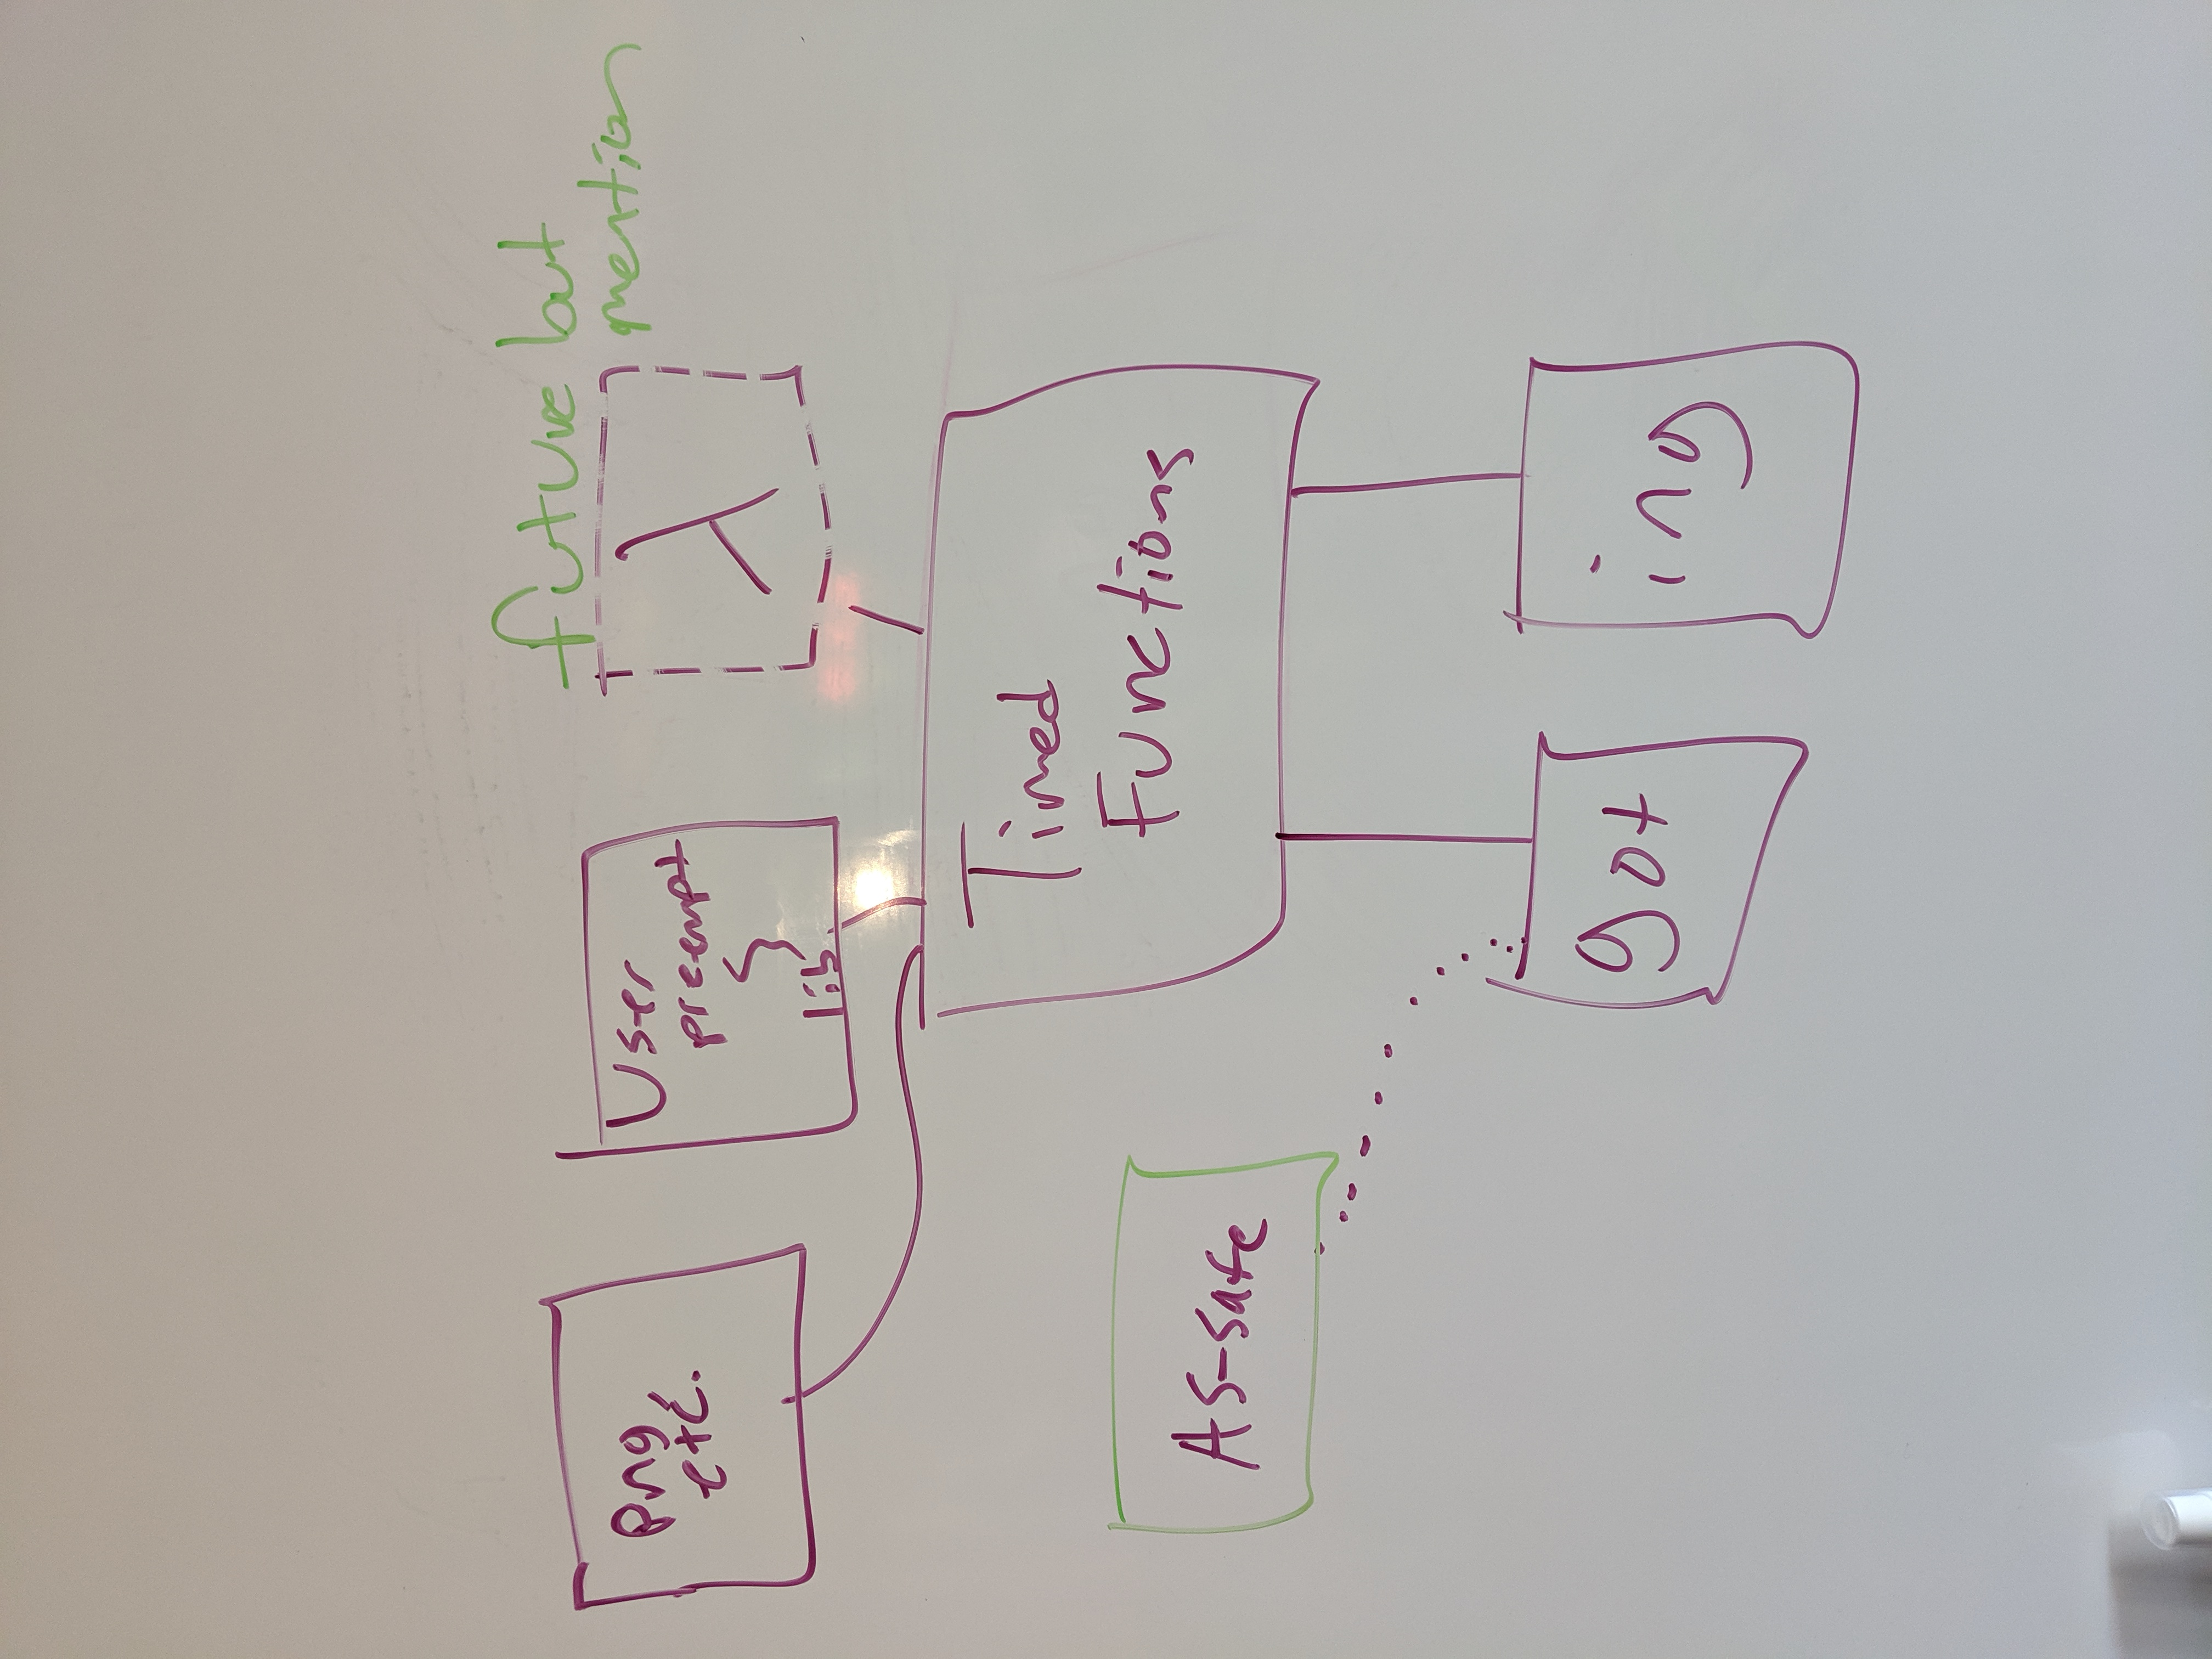
\includegraphics[width=0.75\columnwidth]{figs/architecture}
\end{center}
\caption{The preemptible functions software stack.  \textnormal{Rectangular boxes
represent components implementing the preemptible functions abstraction.  Ovals
represent components built on top of these.  Hexagonal boxes show the
required runtime environment.}}
\label{fig:architecture}
\end{figure}


\subsection{Automatic handling of shared state}

As we found in Section~\ref{sec:intro}, a key design challenge facing
\textit{libinger} is the shared state problem:  Suppose a preemptible function
$\mathcal{F}_0$ calls a stateful routine in a third-party library $\mathcal{L}$, and
that $\mathcal{F}_0$ times out and is preempted by \textit{libinger}.  Later, the
user invokes another timed function $\mathcal{F}_0'$, which also calls a stateful
routine in $\mathcal{L}$.  This constituting a concurrency violation,
\textit{libinger} must hide state modifications in $\mathcal{L}$ by $\mathcal{F}_0$
from the execution of $\mathcal{F}_0'$ to avoid undefined behavior.

The problem is actually even worse.  Those familiar with POSIX signals may notice
that, upon a function's timeout, its caller interrupts it.  \textit{The rest of the
program} can therefore be viewed as a signal handler, and would normally be expected
to restrict itself to calling async-signal-safe (roughly, nonreentrant)
functions~\cite{signal-safety-manpage}.

One non-solution to this problem is to instead prevent preemptible functions from
calling into third-party code (Section~\ref{sec:related}), but doing so would
severely limit their usefulness.  Instead, our approach
is to automatically and dynamically create copies of $\mathcal{L}$ to
isolate state from different timed functions.  Making this work on top of
existing systems software required solving many
design and implementation challenges, which we cover when we introduce
\textit{libgotcha} in Section~\ref{sec:libgotcha}.

\solb{Mention the concurrency implications of the API, and their relation to Rust's
safety guarantees.}


\subsection{Execution stacks}

Recall that, when a preemptible function times out, \textit{libinger} returns a
continuation object.  The caller might pass this object around the program, which
could later call \texttt{resume()} from a different stack frame.  Thus, the
continuation must contain not only the register context, but also the stack
frames belonging to the preemptible function and its callees.  The \texttt{launch()}
function enables this by switching to a new, dedicated stack just before invoking the
user-provided function.

Because of the infeasibility of moving these stacks after a function has started
executing, \textit{libinger} currently heap-allocates large 2-MB stacks so it can
treat them as having fixed size.  The latency of performing these large allocations
was once responsible for an order of magnitude increase in the time overhead of the
\texttt{launch()} operation, so \textit{libinger} now preallocates a large pool of
reusable stacks the first time it is used.


\subsection{Timer interrupts}

\begin{figure}
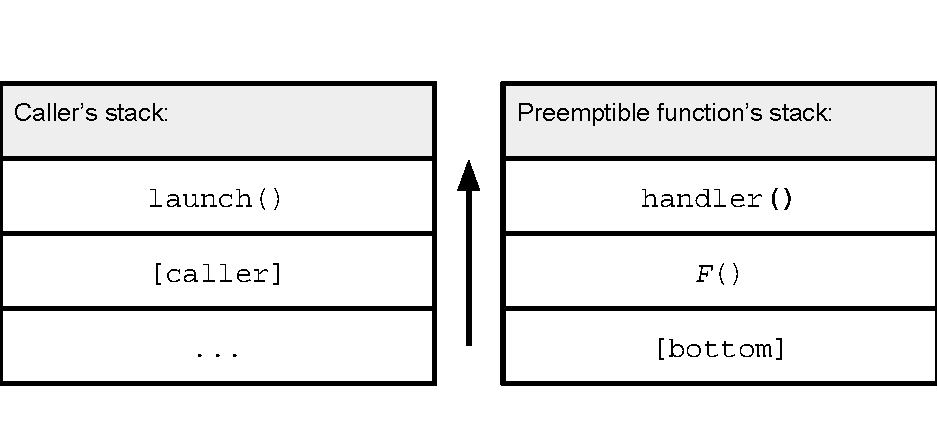
\includegraphics[width=\columnwidth]{figs/twostacks}
\caption{The stacks before and after a timeout.  \textnormal{Upon discovering
that the preemptible function has exceeded its time bound, the handler jumps into the
\texttt{launch()} function.  Then, \texttt{launch()} returns to the original call
site, removing its stack frame in the process.}}
\solb{Remove the continuations from this diagram and add the handler's stack frame.}
\label{fig:twostacks}
\end{figure}

Whenever \textit{libinger} is executing a user-provided function, we
enable fine-grained timer interrupts to
monitor that function's elapsed running time.  A timer interrupt fires
periodically, causing our signal
handler to be invoked each time.  If the function exceeds its timeout,
this handler saves a continuation by dumping the machine's registers.  It then
performs an unstructured jump out of the signal handler and back into the
\texttt{launch()} or \texttt{resume()} function, switching stacks as it does so.
Figure~\ref{fig:twostacks} shows the two stacks of execution
that are present while the
signal handler is running.

A subsequent \texttt{resume()} call restores the registers from the stored
continuation, thereby jumping back into the signal handler.  The handler
returns, resuming the preemptible function from the instruction that was executing
when the preemption signal arrived.

For simplicity, we use a fixed signal frequency for all preemptible
functions, but this is not fundamental to the design.  In the future, we plan to
adjust each function's frequency based on its timeout, and to delay the first signal
until
shortly before the time limit (in the case of longer-running functions).

\solb{THESIS: Removed discussion of our signal pool trick for notifying specific
POSIX threads.}

\solb{THESIS: Removed discussion of our self-signaling trick for restoring a signal
handler's POSIX context without using \texttt{setcontext()}.}


\subsection{Cancellation}

Should a caller decide not to finish running a timed-out preemptible function, it
must deallocate it.  In Rust this happens implicitly via the \texttt{linger\_t}
type's destructor, whereas users of the C interface are responsible for explicitly
calling the \textit{libinger} \texttt{cancel()} function.

Cancellation cleans up the \textit{libinger} resources allocated by
\texttt{launch()};
however, the current implementation
does not automatically release resources already claimed by the
preemptible function itself.  While the lack of a standard resource deallocation API
makes this inherently hard to do in C, it is possible in languages
such as Rust that support destructors.  For instance, the approach proposed by
Boucher et al.~\cite{boucher:atc2018} could be employed to raise a panic
(exception) on the preemptible function's stack.  This in turn would cause the
language runtime
to unwind each stack frame, invoking local variables' destructors in
the process.


\subsection{Performance goals}

\solb{Does any of this section belong in the Evaluation, Future Work, or Conclusion?}

Unlike prior work on low-latency preemptive scheduling such as
Shinjuku~\cite{Kaffes:nsdi2019}, \textit{libinger} runs on top of the existing
OS.  An obvious design to achieve this goal would be to use a thread or a process,
and although we argued in Section~\ref{sec:intro} that such an implementation would
still be far from trivial, our avoidance of these mechanisms has as much to do with
speed.  On Linux, simply spawning a thread incurs an order of magnitude more latency
than our \texttt{launch()} and \texttt{resume()} functions, and forking a process
costs an additional order of magnitude (Section~\ref{sec:eval}).

Recognizing that the asynchrony of interrupting a preemptible function does not imply
inherent asynchrony in accessing its result led us to develop a synchronous
abstraction, thereby obviating the need for the aforementioned spawn operations on
the critical path.  But we deliberately diverged from the design of Shinjuku and RT
in another way as well:\@ unlike these systems, we make each thread responsible for
its own preemption rather than serving preemption signals from a shared watchdog
thread.  This decision was informed by back-of-the-envelope calculations based on
Shinjuku's comparison of the end-to-end latency of bare-metal interprocessor
interrupts (IPIs) versus Linux signals.

While Shinjuku reports that IPIs take an average of only 1,993 cycles, compared to
4,950 for signals (roughly 1:2.5), their sender/receiver breakdown of the latter
number suggests significant latency savings by avoiding cross-core signaling:
First, 343 of those cycles (6.9\%) are spent propagating the signal between the two
cores; we expect this delay to be nearly absent for a timer interrupt originating at
its destination core's own local interrupt controller.  Second, 2,084 cycles (42\%)
are incurred by the sending core; assuming the interrupt controller supports
periodic timer interrupts at the necessary frequency, this cost does not need to be
paid between each interrupt, suggesting measurable savings here too.  Although
our prototype is not yet optimized to this extent, we expect it is possible for a
system built on intra-thread Linux signals to achieve an average preemption latency
within 2x that of Shinjuku's custom operating system.

Of course, in our design, increasing the accuracy of preemption is a tradeoff:\@ more
frequent timer signals mean a tighter bound on timeout detection, but also a lower
throughput of useful work.  The correct balance certainly depends at least on the
timeout value and size of the function, and merits further study.

\solb{THESIS: Could try to confirm these predicted measurements.}

\solb{THESIS: Could explore strategies for choosing POSIX timer intervals.}

\chapter{Resource cleanup and async unwinding: \\ the \textit{ingerc} compiler}
\label{chap:ingerc}

As described so far, one of the facilities that \textit{libinger} enables is
asynchronous function cancellation.  As we saw in Chapters~\ref{chap:functions} and
\ref{chap:safety}, this is a significant achievement that is only possible under the
POSIX safety model thanks to selective relinking.  However, one missing piece of
functionality is automatic cleanup of any resources the cancelled function had
allocated.

The resource leaks associated with cancelling a function are a significant problem:\@
they make cancellation infeasible for long-running applications, which would
experience the cumulative leakage of the resources allocated by all such cancelled
functions.  While a garbage collector would be able to find the leaked resources,
deallocating them might still prove challenging because, without a record of the
interruption point where cancellation occurred, it would not be safe to run object
finalizers.  Of course, our system targets unmanaged languages, so we must accomplish
resource cleanup without a garbage collector.


\section{Languages with unstructured resource management}

In languages such as C, resource lifetimes are completely unstructured, with each
allocation and deallocation performed via an ad-hoc function call.  Some such
functions are well-known because they are prescribed by the C and/or POSIX standards:
\texttt{malloc()}/\texttt{free()}, \texttt{open()}/\texttt{close()}, etc.  However,
applications and libraries can provide their own resource-allocation interfaces, so
it is not possible to identify or track resource management in general.  Worse, there
is no standardization of deallocation functions' interface.  These language
properties mean that automating cleanup would require hand-annotating all custom
allocation and deallocation functions throughout the application and its
dependencies; such annotations would have to provide associations between each
allocator and its corresponding deallocator, as well as information about how to call
the latter.

Were one to build a system to support this, one would need to use an approach like
that of Valgrind's Memcheck~\cite{seward:usenix2005} and LLVM's MemorySanitizer and
instrument the application's allocation and deallocation calls (for which
\textit{libgotcha}'s existing ability to intercept function calls might prove
useful!).  While the memory footprint of this technique is modest compared to that
imposed by \textit{libgotcha}, the runtime slowdown is 3x on memory-intensive
workloads~\cite{stepanov:cgo2015}.  It is probably difficult to dramatically reduce
this overhead because the necessary tracking amounts to adding potentially-expensive
bookkeeping work to each allocation and deallocation, already expensive operations
that can dominate applications' execution.  Worse, the bookkeeping structures need to
be mutable, so care must be taken to avoid designing around data structures with
amortized time complexities, as this would introduce undesirable unpredictable pauses
in preemptible function execution reminiscent of garbage collection\footnote{The
\textit{libgotcha} runtime itself does not suffer from this problem because its
function lookup tables are immutable once process initialization is complete.}.  For
instance, storing allocation records in a hash table would require periodic
rebalancing.

Because of the above limitations, we have not pursued automatic resource cleanup for
preemptible functions written in C.  We advise developers of long-running C
applications to enjoy the other benefits of lightweight preemptible functions, but to
always eventually allow their functions to run to completion.


\section{Languages following the RAII principle}

The situation is more promising in Rust.  Like C++, it adheres to the RAII (Resource
Allocation Is Initialization) idiom that associates each resource's lifetime with
that of some object.  Whenever an object goes out of scope, the program invokes its
destructor and those of its members, freeing the associated resources.  Thus, the
problem of releasing the resources associated with a cancellation can be reduced to
that of invoking the destructors of the objects that are alive at the interruption
point.  Notice that, in contrast to garbage collection, such a model does not divorce
the problem of deallocation from the cancelled function's code; as such, it is not
subject to the safety problems of invoking finalizers, as only the destructors of
objects whose initialization is already complete can be invoked.

Faced with the challenge of safely preempting in the presence of shared state caused
by nonreentrant library interfaces, we found that we could leverage dynamic linking
to solve the problem automatically, and build the \textit{libgotcha} runtime to do
just that.  Here again, we are fortunate to find an existing runtime facility that
can be repurposed to call destructors at an arbitrary position in the program:\@
the Rust language already supports exceptions (which it calls ``panics'').  One
significant advantage to building on top of constructors rather than implementing
separate resource tracking is that exception handling is already designed to add no
overhead to the non-exceptional execution path, which it accomplishes by storing all
necessary information out of band as immutable DWARF debugging annotations stored in
the \texttt{.eh\_frame} section of the ELF object.  With the exception of adding one
cheap function call to each function that owns objects with destructors, we are able
to provide automatic cleanup with no runtime overhead.

\section{Thread library: \textit{libturquoise}}
\label{sec:libturquoise}

\textit{Shinjuku} observes that ``there have been several efforts to implement
efficient, user-space thread libraries.  They all focus on cooperative
scheduling''~\cite{Kaffes:nsdi2019}.  We agree that such libraries are rare, and
attribute this to a lack of natural abstractions to support them.  (Though
\textit{RT} from Section~\ref{sec:related} could be a counterexample, its lack of
nonreentrancy support makes it far from general purpose.)

While the preemptible function is a fundamentally synchronous abstraction, its
simplicity makes it readily composable, and indeed, well-suited to implementing
preemptive threading.  As a proof of concept, we have created a
preemptively-scheduled userland thread library, \textit{libturquoise}\footnote{so
called because it implements ``green threading with a twist''}, by modifying the
\textit{tokio-threadpool}~\cite{www-tokio-threadpool} work-stealing scheduler from
the Rust futures ecosystem.

To migrate the thread pool workers to preemptive scheduling, we made them poll each
task future from within a preemptible function.  We did this in
just 120 new lines of Rust, 50 of them added to version 0.1.16 of the thread library
and
70 spent augmenting \textit{libinger}'s Rust API with a reusable \textbf{preemptible
futures} adapter.

Currently, \textit{libturquoise} assigns each future it launches or resumes the same
fixed time budget, although this design could be extended to support
multiple job priorities.  When a task times out, the scheduler pops it from its
worker thread's job queue and pushes it onto the incoming work queue,
offering it to any available worker for rescheduling after all other waiting jobs
have had a turn.


\subsection{Preemptible futures}

For seamless interoperation between preemptible functions and the futures ecosystem,
we built a preemptible future adapter that wraps the \textit{libinger} API.  This
can be used to pass preemptible functions into a platform designed to process
futures.

Because
of languages' differing futures, this integration is not portable like the core API.
Fortunately, its implementation is a straightforward application of
\texttt{pause()} to propagate cooperative yields across the preemptive function
boundary:\@ we present the general construction of the preemptible future
type and an algorithm for polling one in Listing~\ref{lst:future}.

\begin{figure}
\begin{lstlisting}[label=lst:future,caption=Futures adapter type (pseudocode)]
function PreemptibleFuture(Future fut,
                              Num timeout):
  function adapt():
    while poll(fut) == NotReady:
      pause()
  fut.linger = launch(adapt, 0)
  fut.timeout = timeout
  return fut

function poll(PreemptibleFuture fut):
  resume(fut.linger, fut.timeout);
  if has_finished(fut.linger):
    return Ready
  else
    if called_pause(fut.linger):
      notify_unblocked(fut.subscribers)
    return NotReady
\end{lstlisting}
\end{figure}


\renewcommand{\paper}{chapter\xspace}
\chapter{Microsecond-scale microservices}
\label{chap:microservices}

\ifdefined\chapquotes
\begin{chapquote}{Douglas Adams, \textit{The Hitchhiker's Guide to the Galaxy}}
The ships hung in the sky in much the same way that bricks don't.
\end{chapquote}
\fi

\solb{If this section is too hard to rescue, maybe cut it down and move parts to the conclusion?}

\solb{Probably need to mention JavaScript systems that only require a V8 isolate for each tenant}

This chapter provides a case study of how lightweight preemptible functions could be
used to create the serverless platform of the future.

\begin{namespacereferences}{microservices:}
\input[microservices]{abstract}
\input[microservices]{intro}
\input[microservices]{motivation}
\input[microservices]{isolation}
\input[microservices]{design}
\input[microservices]{design_howclean}
\input[microservices]{eval}
\input[microservices]{future}
\input[microservices]{concl}
\end{namespacereferences}

\renewcommand{\paper}{thesis\xspace}

\section{Conclusion}

We presented the lightweight preemptible function, a composable new abstraction
for invoking a function with a timeout.  This enabled us to build a first-in-class
preemptive userland thread library by implementing preemption atop a cooperative
scheduler, rather than the other way around.  Our evaluation shows that lightweight
preemptible functions have overheads of a few percent (lower than similar OS
primitives), yet enable new functionality.

We believe the lightweight preemptible function abstraction naturally supports
common features of large-scale systems.  For example:  An ad renderer might implement
graceful degradation by rendering frames of an animation in a preemptible function,
dropping unfinished ones to meet its SLO.  An RPC server might preserve work by
processing each request in a preemptible function and memoizing the continuations; if
a request timed out but was later retried by the client, the server could resume
executing it from where it left off.



\backmatter

\chapter{Proposed work}

\solb{Other libinger use:\@ resource limits besides wall-clock time}

\solb{Other libgotcha uses:\@ aspect-oriented programming, multiple library versions}

\begin{swallowsections}
\input[functions]{concl}
\end{swallowsections}


\section{Remaining work}

I propose extending the work already completed in all three of the following ways:

\paragraph{Cancellation resource cleanup for the Rust interface}
Although we currently support asynchronous cancellation of timed-out preemptible
functions via \textit{libinger}'s \texttt{cancel()} facility, we do not yet perform
any automatic cleanup of already-allocated resources.  This is impossible
in general for C programs because the language lacks a destructor mechanism; however,
I intend to add at least partial support for doing so for Rust programs.  The basic
principle will be to throw an artificial exception (Rust panic) on the preemptible
function's execution stack, thereby unwinding the stack and invoking local variables'
destructors.  This approach alone will not guarantee comprehensive cleanup, because
such variables may not have been fully initialized at the time of preemption; for the
same reason, it may have safety ramifications that will merit additional study.  I
have some ideas about how to augment the technique, such as by extending
\textit{libgotcha} to keep a running cache of the several most recent allocations and
deallocations of common resources (e.g., memory and file descriptors) from each
libset.  While exhaustive cleanup may prove difficult to achieve, I hope to at least
catalogue situations where we guarantee not to leak certain classes of resource, and
perhaps provide a tunable allowing users to request full resource tracking if needed.

\paragraph{Automatic selection and variation of timer frequency}
For simplicity, the current \textit{libinger} implementation subscribes to timer
signals spaced a globally constant interval apart throughout the entire duration of
each preemptible function.  To improve efficiency while preserving preemption
granularity, I plan to dynamically determine this interval based on the requested
timeout.  For long-running functions, this will include delaying the first of these
signals until shortly before the timeout would expire.  Maintaining accuracy across
multiple CPUs will probably require building in a calibration routine to infer
configuration parameters.

\paragraph{Support OpenSSL and benchmark hyper with HTTPS}
Earlier in \textit{libgotcha}'s development history, it was able to run nginx with
OpenSSL.  Recent attempts at getting hyper to run with OpenSSL have ended in crashes,
yet this configuration is desirable for measurement because it exhibits a far greater
number of dynamic function calls, of which \textit{libgotcha} alters the performance
characteristics.  I aim to support and benchmark the configuration, which will likely
involve regression testing using the old nginx setup.

\hfill \\
\noindent
Additionally, I will complete one of the following projects, as selected by the
committee:

\paragraph{Achieve even finer--grained preemption}
The \textit{Shinjuku} authors included IPI microbenchmarks that suggest it should be
possible for us to achieve interrupt latencies and spacing within a small constant
factor of theirs.  I could attempt to achieve this by reusing some of their
optimizations to POSIX contexts and adding a specialized timer signal delivery
mechanism to the kernel to reduce the number of ISR instructions at the expense of
generality.

\paragraph{Implement ``\textit{libingerOS}'' container framework}
Generalizing the serverless platform case study, it should be possible to generate a
utility that takes two or more position-independent executables and combines them
into a single process whose thread(s) are timeshared between the ``programs'' using
preemptible functions.  Obviously, this would only provide memory isolation for
programs implemented in memory-safe languages.  This would be implemented on top of
\textit{libinger} as a sample application.

\paragraph{Implement a caching RPC framework}
The preemptible functions API naturally lends itself to problems of caching partial
computations, and one interesting case study would be a caching RPC framework.  I
imagine this working as follows:  Clients would enclose alongside each request the
timeout they were using when listening.  The server would process each request inside
its own preemptible function.  When the client timed out waiting for a response, the
server would simultaneously time out and cache the continuation.  Subsequent requests
for the same procedure with identical inputs would resume the interrupted computation
from where it left off.


\section{Timeline}

\begin{itemize}
\item 24 April 2020: ATC '20 author notification
\item 4 June 2020: ATC '20 camera-ready deadline (if applicable)
\item June 2020: Start cancellation resource cleanup, fix OpenSSL support
\item July 2020: Continue cancellation resource cleanup, fix OpenSSL support
\item August 2020: Finish cancellation resource cleanup
\item September 2020: Speaking skills talk, start automatic preemption intervals
\item October 2020: Finish and evaluate automatic preemption intervals
\item November 2020: Start committee-selected project
\item December 2020: Finish and evaluate committee-selected project
\item January--March 2021: Thesis writing, run any final experiments
\item April 2021: Finish thesis
\item May 2021: Defense
\end{itemize}


\cleardoublepage
\addcontentsline{toc}{chapter}{Bibliography}
\bibliography{ref}

\end{document}
